\documentclass[journal]{IEEEtrancz}
% zvolte kodovani
\usepackage[utf8]{inputenc} % linux/unix
%\usepackage[latin2]{inputenc}
%\usepackage[cp1250]{inputenc} % Windows
\usepackage[czech]{babel}
\usepackage{graphicx}

\begin{document}

\title{Comparing various approaches to the mTSP problem}
\author{Teymur Azayev}

\maketitle

\begin{abstrakt}
We take a look at the mTSP problem and compare various approaches to finding approximate solutions, including local search, evolutionary algorithms, and an memetic search.
\end{abstrakt}


\IEEEpeerreviewmaketitle

\section{Task}
The task is to find an approximate solution to a variant of the Travelling Salesman Problem using local search and evolutionary algorithms and to compare the results of the algorithms.

\section{Introduction}
The Travelling Salesman Problem (TSP) is a task where given a number of cities we are looking for the shortest path that we can take while visiting all the cities only once and ending up at the city where we started at. 
This task can also be formalized as finding the shortest tour in a weighted non-oriented graph. \\
The mTSP task is a generalization to the TSP where we have multiple agents
The mTSP, as the vanilla TSP problem are inherently NP-hard. We therefore have to use various approximate
optimization techniques which help us find an 'acceptable' solution to the problem.

\section{Goals}
The point of this report is to compare and benchmark local approaches with evolutionary algorithms in the mTSP
problem, and to discuss how various issues have been dealt with along the way. We also hope that by comparing the various approaches we will get an insight to the nature of the problem.

\section{Implementation}
The problem is given by $n$ cities and $m$ agents. There is also an auxilliary city called the depot. Every agent
starts from and finishes at the depot. The solution is represented by two parts: A sequence of cities and a pair of boundaries for each agent. Each agent starts at the depot, then proceeds sequentially through the solution, beginning his boundary start index and finishing at his boundary stop index. From there the agent goes back to the depot. \\
The quality of the solution (and the fitness function) is taken as the longest route of all agents. This not only implicitly takes into account the total length of all tours of the agents, but normalizes the tour lengths so that they all approximately cover the same distance. We generate a concrete problem by randomly generating n points within a reasonable distance from the origin. We then run the algorithm and evaluate the solution after a certain amount of iterations. \\
As mentioned in the abstract, we use three different approaches to finding solutions for the mTSP.
The first approach is a simple local search algorithm. At every iteration we perform the following. We swap two of the cities in the sequence, evaluate the fitness and swap it back to how it was. This is done $n$ times
and the 'best swap' is recorded out of that iteration. The best swap is then performed and saved. \\
We also use an improved version of the local search algorithm where we perform a series of swaps and then keep only the best swap. This allows for solution worsening and as we will see in the results, performs better than the first version.
The second approach is a basic evolutionary algorithm on the same representation of the problem. 
A population of 300 individuals is used at every iteration. The parents are selected using a standard roulette approach and two new offspring are created using a one-point crossover operator. In each generation we select a tenth of the population to create new offspring. In order to produce a valid  every time we need to slightly modify the crossover operator. This is done by the offspring receiving part of the solution from one parent and sequentially recieving the rest of the sequence from the other parent such that the final sequence is valid. As a mutation, in each iteration we allow the boundaries of each agent to change with chance, meaning that each agent can have fewer or more cities in their path. The mutation rate is set to about 5\%. The new offspring are accepted if they are better than their parents and accepted with a small chance if they are worse. \\
The last approach, the memetic algorithm simply extends the evolutionary algorithm by a local search at each iteration. This is done by using 2-opt on randomly chosen individuals from the population at each generation after the new individuals have been created. This is a method to let weak individuals locally improve and give them a chance to be selected in the next evaluation.


\section{Experiments}
The initial experiments have been done on randomly generated graph to validate and compare the three algorithms.
To make a fair comparison, however, we use the provided benchmark graph and evaluate the algorithms on that benchmark. We use a total of 10 repetitions take the average score and progress of each algorithm which we will then compare. In figure \ref{fig:progfig} we can see an iteration plot of all four algorithms to get 
a visual understanding and comparison of the progress of each algorithm. We can see that the local algorithm
converges to a local solution almost immediately and does not continue to improve. Due to implementation reasons we do not consider execution times of each algorithm, but rather the iterations that they takes. 
During the tuning phase of the algorithms a fitness histogram was plotted it was noted that the population converges prematurely, leading to local minima. To attempt to combat this we used a higher population size and linear fitness scaling, but this did not entirely eliminate the problem.


\begin{figure}[ht]
  \centering
    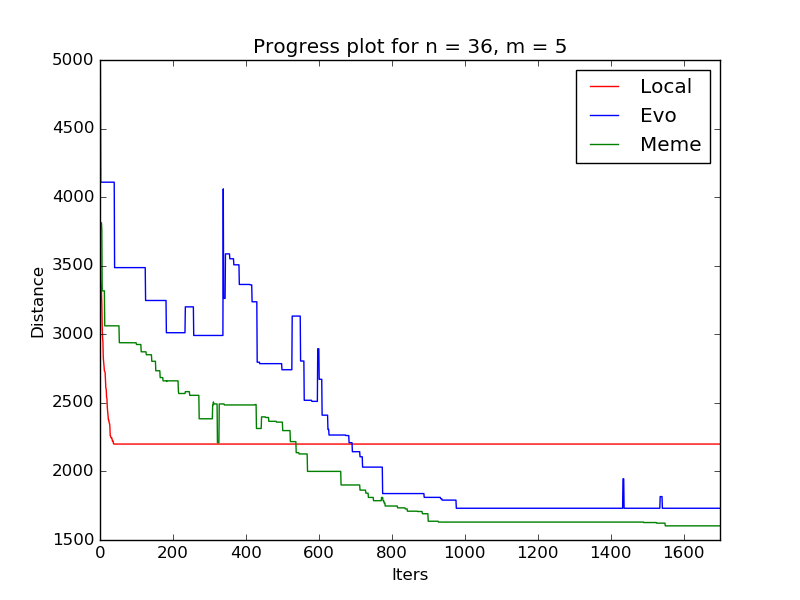
\includegraphics[width=9cm]{progplot}
      \caption{Progress plot of each algorithm}
    \label{fig:progfig}
\end{figure}

\begin{figure}[ht]
  \centering
    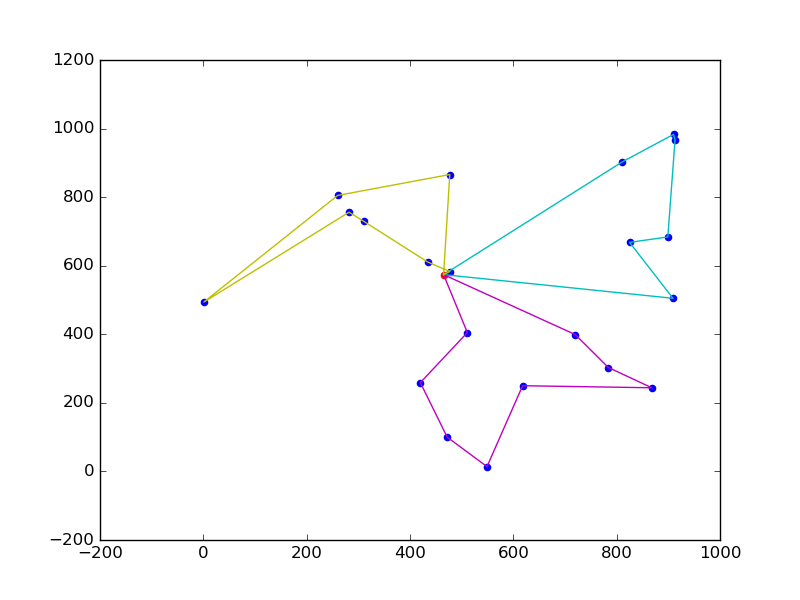
\includegraphics[width=9cm]{clean}
      \caption{Visual solutions of n = 22, m = 3}
    \label{fig:solfig}
\end{figure}


\begin{table}
  \centering
  \caption{Average scores of the three algorithms}
  \begin{tabular}{|l||c|c|c|c|}
  \hline
    & Local & Local imp & Evolution & Memetic\\
  \hline
  \hline
  Distance of largest tour  & 6411 & 5100 & 5161 & 5194 \\
  \hline
  \end{tabular}
  \label{tab:extab}
\end{table}


\section{Discussion}
As expected, the local search converged immediately and did not improve further. The improved local search (similar to simulated annealing) performed best.
The evolutionary algorithms proved difficult to train as the population converged prematurely to a local minimum. This is a common problem in EA and is mediated by a few different methods. We attempted to increase population and modify the selection/replacement strategy, as well as applying linear fitness scaling to provide the necessary selection pressure. This improved the solution, but still led to premature convergence. This could be seen by plotting a fitness histogram at each iteration. The standard evolutionary algorithm took much longer to train but got comparable results. The memetic algorithm performs on average similarly to the evolutionary algorithm, this is probably due to the inadequately chosen fitness or due to the 2-opt not being performed that often given that it is very expensive to compute unless a sofisticated implementation is used. Results could most likely be further improved by tuning the evolutionary algorithm hyperparameters such as population size, mutation rate, etc. \\


\section{Conclusion}
We have seen that a simple local search and evolutionary algorithm can give us reasonable approximate solutions to an np-hard problem such as the mTSP. These types of approaches are credited because they are relatively simple to implement. For a large amount of cities, however, this algorithm has trouble working out of the box and can be very slow so it requires an efficient implementation and more hyperparameter tuning.


\end{document}
